Este capítulo tem o objtivo de apresentar como se pode realizar a execução de testes da gema de
exemplo ‘‘\emph{gemtranslatetoenglish}''. Na seção \ref{section:teste_com_rake}, apresentaremos
como é feita a execução de testes com o \emph{rake}, e apresentaremos na seção
\ref{section:teste_com_irb}, como realizar testes com a ferramenta \emph{irb}.


\section{Testes com rake}
\label{section:teste_com_rake}


Esta seção tem o objetivo de mostrar como se pode realizar os teste, após criar os códigos de
funcionalidade, visto na sub-seção \ref{subsection:codigo_de_funcionalidade_no_diretorio_lib}, e os códigos
de teste, visto na sub-seção \ref{subsection:codigo_de_teste_no_diretorio_test_ou_spec}.

Antes de realizarmos os testes, precisamos criar a gema com comando \textbf{‘‘\emph{gem build 'nome da gema'.gemspec}''}
e fazer a instalação com o comando \textbf{‘‘\emph{sudo gem install 'nome da gema'-'versão da gema'.gem}''}. 

No nosso exemplo, foi fazer a execução dos comandos mostrados no código
\ref{lst:execucao_que_cria_e_instala_gemtranslatetoenglish} para fazer a criação e a instalação da gema
‘‘\emph{gemtranslatetoenglish}''.

\lstinputlisting[ style=customBash, caption={Execução que Cria e Instala gemtranslatetoenglish}, label={lst:execucao_que_cria_e_instala_gemtranslatetoenglish}]
{codigos/execucao_que_cria_e_instala_gemtranslatetoenglish.sh }

Agora após ter implementado o código das funcionalidades, o arquivo de teste
‘‘\emph{test/test\_check\_translate.rb}'', o arquivo \emph{Rakefile}, e ter feito a criação e a instalação
da gema de exemplo, podemos realizar os testes com a execução do comando ‘‘\emph{rake}'' no terminal.

Com a execução dos testes, obtemos como resultado o código \ref{lst:execucao_rake_gema_gemtranslatetoenglish},
explicado logo a seguir.

\lstinputlisting[ style=customBash, caption={Execução rake gema gemtranslatetoenglish}, label={lst:execucao_rake_gema_gemtranslatetoenglish}]
{codigos/execucao_rake_gema_gemtranslatetoenglish.sh }

\begin{itemize}

 \item Na linha ‘‘1'' é feito a execução do comando ‘‘\emph{rake}'' para se realizar os testes.

 \item Na linha ‘‘5'' é mostrado que foram feitos 2 testes, no caso os 2 que definimos no código
 \ref{lst:test_check_translate.rb} nas linhas ‘‘8'' a ‘‘11'' no teste ‘‘\emph{test\_world\_translation}''
 e nas linhas ‘‘12'' a ‘‘15'' no teste ‘‘\emph{test\_text\_translation}''. Também é apresentado na
 linha ‘‘5'' que foram feitos 4 ‘‘\emph{assertions}'', no caso dois para cada caso de teste feitos por
 meio do ‘‘\emph{assert\_equal}''. E além disso é apresentado que não ocorreram  \emph{failures}'',
 ‘‘\emph{errors}'' e ‘‘\emph{skips}''.

\end{itemize}

Deste modo, ao se realizar estes testes garantimos que pelo menos a função ‘‘\emph{translate()}'' da gema
‘‘\emph{gemtranslatetoenglish}'', esta funcionando como o esperado.


\section{Testes com irb}
\label{section:teste_com_irb}


Esta seção tem o objetivo de mostrar como se realiza teste utilizando a ferramenta \emph{irb} que permite
verificar as funcionalides de uma gema de forma manual, sem a necessidade de inclui-lá em um projeto.

O \emph{\href{http://www.ruby-doc.org/stdlib-2.0/libdoc/irb/rdoc/IRB.html}{IRB}} 
\footnote{IRB: \url{http://www.ruby-doc.org/stdlib-2.0/libdoc/irb/rdoc/IRB.html}}
(\emph{Interactive Ruby Shell}) é uma ferramenta do \emph{Ruby} que serve para executar expressões
interativamente, fazendo a leitura da entrada padrão [\citeonline{irb_doc}].

%Caso se deseje fazer os testes de uma gema manualmente podemos
%fazer o uso do ‘‘\emph{IRB}'', chamando o comando ‘‘\emph{irb}''.
% o seguinte comando mostrado no código ‘‘Código \ref{lst:executa_irb} - Executa IRB'' no terminal para iniciá-lo.

\begin{comment}
\lstinputlisting[ style=customBash, caption={Executa IRB}, label={lst:executa_irb}]
{codigos/executa_irb.sh}
\end{comment}

Um exemplo de uso do \emph{IRB} pode ser visto 
% na imagem ‘‘Figure \ref{fig:exemplo_de_uso_do_irb} - Exemplo de Uso do IRB'' 
no código \ref{lst:exemplo_de_uso_do_irb}
abaixo, explicado em mais detalhes na listagem abaixo. 

\begin{comment}
\begin{figure}[ht]
  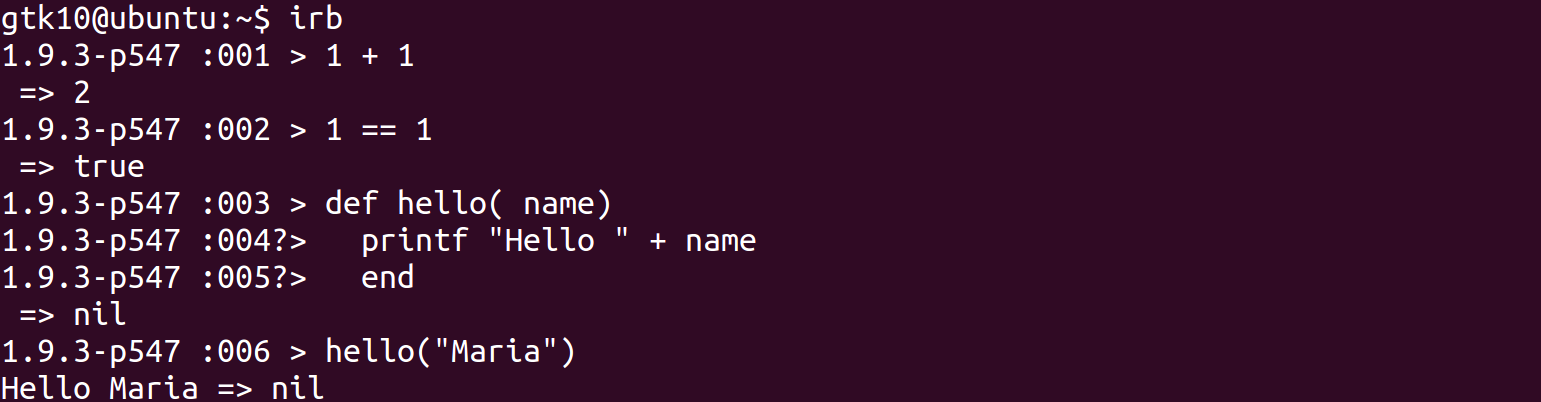
\includegraphics[scale=0.3]{images/exemplo_de_uso_do_irb}
  \caption{Exemplo de Uso do IRB}
  \label{fig:exemplo_de_uso_do_irb}
\end{figure}
\end{comment}

\lstinputlisting[ style=customBash, caption={Exemplo de uso do IRB}, label={lst:exemplo_de_uso_do_irb}]
{codigos/exemplo_de_uso_do_irb.sh}

\begin{itemize}

\begin{comment}
 \item Primeiramente é feita a chamada da ferramenta \emph{IRB} com o comando ‘‘\emph{irb}'' no terminal.
 
 \item Depois é requisitado a soma entre ‘‘\emph{1 + 1}'' resultando em ‘‘\emph{2}''.
 
 \item Em seguida é perguntado se ‘‘\emph{1 == 1}'' resultando em ‘‘\emph{true}''.

 \item E no fim é criado uma função chamada de ‘‘\emph{hello}'' com o parâmetro ‘‘\emph{name}'' e ao se 
 chamar essa função é devolvido na tela ‘‘\emph{Hello +}'' o parâmetro passado para a função. O resultado
 pode ser visto quando se requisita ‘‘\emph{hello(‘‘Maria'')}'' e se obtem como resultado 
 ‘‘\emph{Hello Maria}''.
\end{comment}
 
  \item Primeiramente na linha ‘‘1'' é feita a chamada da ferramenta \emph{IRB} com o comando ‘‘\emph{irb}'' 
  no terminal.
 
 \item Depois na linha ‘‘2'' é requisitado a soma entre ‘‘\emph{1 + 1}'' resultando em ‘‘\emph{2}'' na linha 
 ‘‘3''.
 
 \item Em seguida na linha ‘‘4'' é verificado se ‘‘\emph{1 == 1}'' resultando em ‘‘\emph{true}'' na linha 
 ‘‘5''.

 \item E no fim entre as linhas ‘‘6'' e ‘‘8'' é criado uma função chamada de ‘‘\emph{hello}'' com o 
 parâmetro ‘‘\emph{name}'' e ao se chamar essa função é devolvido na tela ‘‘\emph{Hello}'' mais o 
 parâmetro passado para a função. O resultado pode ser visto quando se requisita 
 ‘‘\emph{hello(‘‘Maria'')}'' na linha ‘‘10'', obtendo como resultado ‘‘\emph{Hello Maria}'' na linha ‘‘11''.
 
\end{itemize}

No nosso exemplo da gema ‘‘\emph{gemtranslatetoenglish}'' fizemos alguns testes simples mostrados
na código \ref{lst:teste_irb_da_gema_gemtranslatetoenglish} explicado com mais detalhes nos itens abaixo.

\begin{comment}
\begin{figure}[ht]
  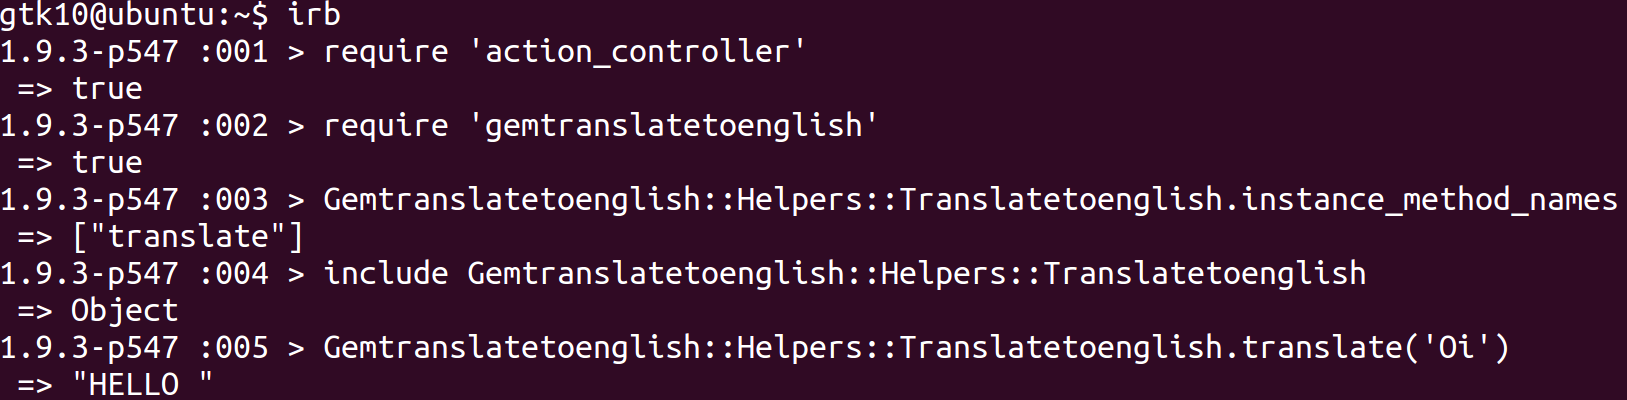
\includegraphics[scale=0.28]{images/teste_irb_da_gema_gemtranslatetoenglish.png}
  \caption{Teste IRB da gema gemtranslatetoenglish}
  \label{fig:teste_irb_da_gema_gemtranslatetoenglish}
\end{figure}
\end{comment}

\lstinputlisting[ style=customBash, caption={Teste IRB da gema gemtranslatetoenglish}, label={lst:teste_irb_da_gema_gemtranslatetoenglish}]
{codigos/teste_irb_da_gema_gemtranslatetoenglish.sh}

\begin{itemize}

 \item Primeiramente na linha ‘‘1'' é feita a chamada da ferramenta \emph{IRB} com o comando ‘‘\emph{irb}'' 
  no terminal.
  
  \item Na linha ‘‘2'' é executado o comando ‘‘ \emph{require 'action\_controller'} '' para buscar a gema 
  ‘‘\emph{ActionController}'' necessária no uso da nossa gema de exemplo quando evitamos digitar a 
  \emph{PATH} completa na ‘‘\emph{view}''.

  \item Na linha ‘‘4'' é executado o comando ‘‘ \emph{require 'gemtranslatetoenglish'} '' para buscar a 
  nossa gema de exemplo.
  
  \item Na linha ‘‘6'' é executado o comando 
  ‘‘ \emph{instance\_method\_names}'' para verificar se o nosso método \emph{translate()} existe.
  
  \item Na linha ‘‘8'' é executado o comando ‘‘\emph{include}'' para incluir as funções do módulo 
  ‘‘\emph{Translatetoenglish}''.
  
  \item Na linha ‘‘10'' é executado o comando 
  ‘‘\emph{translate('Oi')}'' para verificar se a função funciona como o esperado.
  
  \item E no fim na linha ‘‘11'' podemos verificar que a função \emph{translate()} funcionou corretamente,
  pois obtemos como resultado a palavra ‘‘\emph{HELLO }''.
  
 \end{itemize}